\chapter{基于消息传输收益的最优队列调度算法}
\label{chap:基于消息传输收益的最优队列调度算法}

本章尝试改进经典的基于概率预测的路由算法PRoPHET \cite{AndersLindgren2004}。定义了“传输收益”概念,基于此,提出了传输收益最优化,吞吐量相关的概率路由问题(Optimal Throughput-Aware Probabilistic Routing)。该问题被建模为最优决策问题,并在本章中采用动态规划方法解决。在该模型下,提出了一种数据项选择机制,其具有如下特点:
\begin{enumerate}
\item 每一对节点所对应的潜在连接,其平均数据吞吐量可能比缓存中的消息大小要小。
\item 每次传输的能量消耗不可忽略,换言之,消息传输不成功会带来无收益的能量损耗。
\end{enumerate}

例如,针对某条消息的一次传输操作而言,若当前连接所允许的总数据量比消息的大小小很多,则该次传输终止时,消息并未被成功传输。针对该问题的一个解决办法,即是总是传输不超过该连接平均吞吐量大小的消息,从而避免浪费传输机会。退一步而言,即使连接的吞吐量完全足够传输每一条消息,传输不同消息所带来的收益也并不相同(比如投递率收益,及投递时延收益等),然而传输的机会是有限的,故针对每一次传输机会而言,传输不同的消息对路由的整体性能表现具有较大的影响。从这个角度而言,在机会网络中,为了提高路由性能表现,应当设计有效的数据项选择机制。

本章组织如下:\ref{chap4:系统模型}节中介绍了系统模型及路由模型;\ref{chap4:问题形式化}节中形式化定义了关键问题;\ref{chap4:基于数据项选择的改进路由}节中利用设计的数据项选择机制对PRoPHET进行改进;\ref{chap4:仿真实验}节为仿真实验;\ref{chap4:本章小结}节概括了本章内容。

\section{系统模型}
\label{chap4:系统模型}

\begin{table*}
\centering
  \caption{数学符号}
    \label{tab:chap4_notations}
  \begin{tabular}{p{0.23\linewidth}<{\centering}p{0.7\linewidth}<{\centering}}
  \hline
    \textbf{Notation} & \textbf{Meaning}  \\
    \hline
   $\mathcal{N}$ & 网络节点集合 \\
   $n_i$ &  第 $i$ 号节点  \\
   $m_i$ &  第 $i$ 号消息 \\
   $TTL(i)$ & 消息 $m_i$ 的生存时间\\
   $S(i)$   & 消息 $m_i$ 的大小\\
    $\zeta(i)$ & 消息 $m_i$ 的传输收益\\
    $B_{(a,b)}$ & 节点 $n_a$ 与 $n_b$ 之间的带宽\\
   $t_{s_{(a,b)}}/t_{e_{(a,b)}}$   &  节点 $n_a$ and $n_b$ 最近一次连接的开始/结束时间\\
   $\tau_{a,b}$ & 节点 $n_a$ 与 $n_b$ 预测接触时间\\
  $P_{(a,b)}$ & $n_a$'s 节点 $n_a$ 与 $n_b$ 的预测接触概率 \\
  $ETH_{(a,b)}$ & 节点 $n_a$ 与 $n_b$ 连接的预测吞吐量\\
$P^{\{a,b\}}$ & 节点 $n_a$ 与 $n_b$ 的共同投递率\\
   \hline
  \end{tabular}
\end{table*}

数学符号如\tablename~\ref{tab:chap4_notations}所示。本模型的时间线设为离散时间,时间轴被划分为多个小的时间槽,每个时间槽的长度定义为一个单位时间。整个节点集合用符号$\mathcal{N}=\{n_i|n_i\in\mathcal{N},1\leq i<|\mathcal{N}|\}$。对于任意一条消息$m_k$,其消息生存时间表示为$TTL(k)$。当消息$m_k$被某节点产生时,$TTL(k)$的值即被指定。若某条消息的$TTL$到期,则消息会被当前节点丢弃。消息$m_k$的大小用符号$S(k)$表示。模型假设任一节点$n_i$知道其自身接口的带宽$B(i)$。该假设的合理性建立在网络中的每个节点往往在通信时都采用统一标准的某种接口,如蓝牙,wifi等。退一步讲,即使接口状态不稳定,也可以利用滑动窗口法对其平均值进行预测。对于任意一对相遇节点$n_i$及$n_j$,令节点$n_i$记录两个值$t_{s_{(i,j)}}$及$t_{e_{(i,j)}}$,分别用于记录两节点间最近一次连接的开始时间及结束时间。于是$t_{e_{(i,j)}}-t_{s_{(i,j)}}$即代表该次连接的持续时间;为简单起见,符号$t_{s_{(i,j)}}$及$t_{e_{(i,j)}}$在无歧义的上下文中,简记为$t_s$和$t_e$。

PRoPHET路由算法\cite{AndersLindgren2004}记录了节点的相遇历史,用于预测节点间的相遇概率,并且考虑到了相遇概率具有传递性的特点。在PRoPHET中,$P_{(a,b)}$即用于衡量节点$n_a$及$n_b$之间投递概率的效用函数,存于节点$n_a$内。$P_{(a,b)}$的计算及更新方法如下式所示。

\begin{equation}
P_{(a,b)}=P_{(a,b)_{old}}+(1-P_{(a,b)_{old}})\times P_{init}
\label{eq:prophet1}
\end{equation}
\begin{equation}
P_{(a,b)}=P_{(a,b)_{old}}\times\gamma^{k}
\label{eq:prophet2}
\end{equation}
\begin{equation}
P_{(a,c)}=P_{(a,c)_{old}}+(1-P_{(a,c)_{old}})\\
\times P_{(a,b)}\times P_{(b,c)}\times \beta
\label{eq:prophet3}
\end{equation}

其中,$P_{init}$, $\beta$及$\gamma$是位于$[0,1]$范围内的常数。每个节点维护一个$1\times|\mathcal{N}|$的向量,该向量中第$i$个元素记录了节点$n_a$对节点$n_i$的投递率。

\section{问题形式化}
\label{chap4:问题形式化}

本节给出问题的形式化定义。

\subsection{问题目标}
问题目标即是最大化每条消息的投递概率。在机会网络中,每个节点以“存储-携带-转发”的方式对消息进行路由。在机会路由中,一种策略是总是让节点选择对目的节点投递率高的消息进行投递。吞吐量与节点间的接触时间及通信接口带宽具有很强的相关性,因此对消息是否能投递成功具有较大的影响。然而在该种方法中,节点之间连接的吞吐量因素并未考虑进去。由于节点的带宽,接触时间及接触机会非常有限,缓存消息队列的调度策略对路由性能表现具有很大的影响。假设节点$n_a$持有三条消息$m_i$, $m_j$及$m_k$,其目的节点都为$n_b$,大小分别为150 K, 200 K 与100 K。然而当前连接最多只能传输120 K 的数据量。在此情况下,由于连接吞吐量的限制,消息$m_i$和$m_j$都无法被成功传递。一种做法是让$n_a$按消息大小从小到大传递,然而这种方法虽然能保证部分消息成功传输,但并未设定任何优化目标,由此可能使得某些虽然大小稍大,但也能成功传递,且对投递率具有较大改进的消息无法充分利用该次机会传输。为解决此问题,需要对消息的调度设定一个可行的评估指标。在本章中,主要集中研究如何有效的数据项选择机制提高消息的投递率。下面将给出最优化消息传输投递率收益的分析过程。

若消息被节点$n_a$转发给$n_b$,则该消息宣告传输失败,仅当$n_a$及$n_b$都未成功传输该消息,其投递率可以用公式(\ref{eq:probability})计算。

\begin{equation}
P^{\{a,b\}}=1-(1-P_{(a,d_i)})(1-P_{(b,d_i)})
\label{eq:probability}
\end{equation}

于是对于传输收益有如下定义。

\begin{definition}传输收益.\\
传输收益函数$\zeta(i)$用于衡量消息$m_i$在本次传输过程中能够改善的投递率, 有
\begin{equation}
\zeta(i)=P^{\{a,b\}}-P^{\{a\}}\\
=1-(1-P_{(a,d_i)})(1-P_{(b,d_i)})-P_{(a,d_i)}
\label{eq:improve}
\end{equation}
\end{definition}

函数$\zeta(i)$的值代表将消息$m_i$从节点$n_a$传输给节点$n_b$所带来的投递率收益。从这点出发,可以如下定义“吞吐量相关最优机会路由”概念。

\begin{definition} 吞吐量相关最优机会路由. \\
最优机会路由总是尝试最大化消息投递概率,且考虑带宽及接触时间两个因素。节点$n_i$将依照$\zeta$函数值选择消息传输给节点$n_j$,利用预测的吞吐量最大化$\zeta$值总和。
\label{def:throughput-routing}
\end{definition}

例如,在\tablename~\ref{tab:chap4_zeta} 所示例子中,节点$n_a$缓存中总共有5条消息,记为$m_1$, $m_2$, $m_3$, $m_4$, $m_5$。消息$m_i$的目的节点记为$d_i$。对于其中任意一条消息$m_i~(1\leq i\leq 5)$,有$P_{(b,d_i)}>P_{(a,d_i)}$。在这种情形下,当节点$n_a$与$n_b$相遇时,所有这5条消息都应由$n_a$转发给$n_b$。由公式~(\ref{eq:improve})可以得到每条消息对应的$\zeta$值。在下一小节中,将给出吞吐量的预测方法,然后给出问题的形式化定义。

\begin{table}
\centering
  \caption{节点$n_a$缓存中的5条消息}
  \label{tab:chap4_zeta}
  \begin{tabular}{cccccc}
  \hline
    data item  & $m_1$ & $m_2$ & $m_3$ & $m_4$ & $m_5$ \\
    \hline
    $P_{(a,d_i)}$ & 0 & 0.2 & 0.1 & 0.12 & 0.2 \\
    $P_{(b,d_i)}$ & 0.1  & 0.75  & 0.2 & 0.25 & 0.35  \\
    value of $\zeta$ & 0.1 & 0.6 & 0.18 & 0.22 & 0.28 \\
    message size & 1K  & 2K  & 5K   & 6K   & 7K   \\
    \hline
  \end{tabular}
\end{table}

\subsection{吞吐量预测}
\label{sec:吞吐量预测}

\begin{definition}连接吞吐量. \\
给定任意两个节点的接触时间 $t$,以及带宽 $B$ (KB/unit) , 该次连接的吞吐量,记为 $TH$ ,有
\[
TH=B\cdot t
\]
\label{def:throughput}
\end{definition}

\begin{figure}
  \centering
  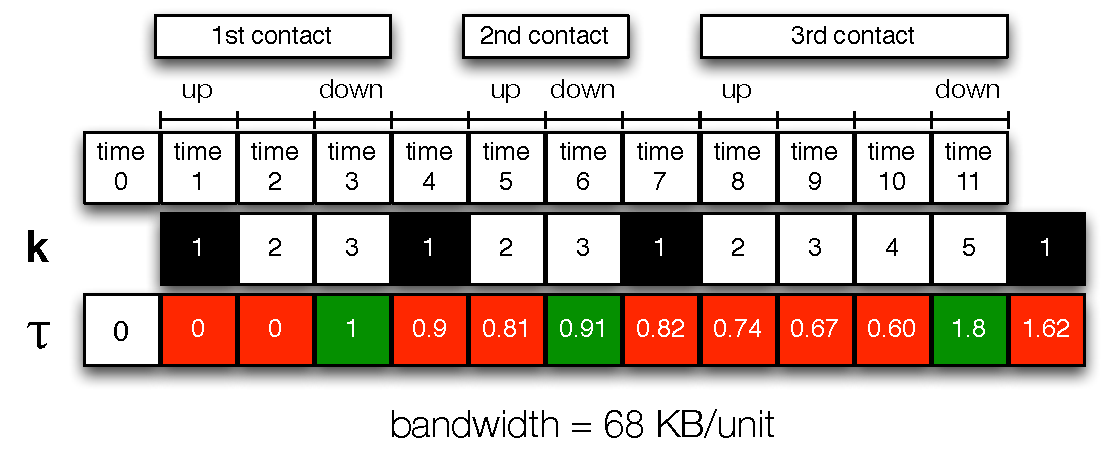
\includegraphics[width=0.8\textwidth]{paper-data/example2}
  \caption{带宽预测过程}
  \label{fig:chap4_example2}
\end{figure}

在此假设带宽$B$为已知,要预测吞吐量,则只需预测出连接的持续时间$t$。采用公式~(\ref{eq:estimate})~预测下一次$n_a$与$n_b$之间连接的持续时间。
\begin{equation}
\tau_{(a,b)_{new}}=(1-\alpha)\tau_{(a,b)_{old}}+\alpha(t_e-t_s)
\label{eq:estimate}
\end{equation}
其中$\alpha\in[0,1]$是常数参数,$t_e-t_s$是节点$n_a$与$n_b$之间最近一次连接的持续时间,该部分加权为$\alpha$。当$\alpha$值设的较大时,公式~(\ref{eq:estimate})后半部分的影响较大,反之亦然。

当节点$n_a$一段时间内没有再与节点$n_b$接触时,则用公式~(\ref{eq:estimate2})更新$\tau_{(a,b)}$。
\begin{equation}
\tau_{(a,b)_{new}}=\tau_{(a,b)_{old}}\gamma^{k}
\label{eq:estimate2}
\end{equation}
其中$\gamma\in[0,1)$是衰减常数,如公式~(\ref{eq:prophet2})一样;$k$是离上一次更新公式流逝的单位时间数目(即经过的时间槽数目)。

在每个时间槽内,对于任意一对节点$n_a$和$n_b$,在每一个时间槽,节点都会检查$n_a$及$n_b$的连接状态。对$\tau$的更新过程如算法~\ref{alg:chap4_estimate}所示。根据定义~\ref{def:throughput}~所示关于$n_a$与$n_b$之间吞吐量的定义,吞吐量可以由公式~(\ref{eq:eth})预测。

\begin{algorithm}[tbp] %算法的开始
\renewcommand{\algorithmicrequire}{\textbf{For}}
\caption{Updating the $\tau$ value} %算法的标题
\label{alg:chap4_estimate} %给算法一个标签,这样方便在文中对算法的引用
\begin{algorithmic}[1] %这个1 表示每一行都显示数字
\REQUIRE the current time unit
\IF{connection is up}
    \STATE $t_s\leftarrow current\_time$
    \STATE $\tau_{(a,b)_{new}}=\tau_{(a,b)_{old}}\gamma^{k}$
    \STATE $k\leftarrow k+1$
\ELSIF{connection is down}
    \STATE $t_e\leftarrow current\_time$
    \STATE $\tau_{(a,b)_{new}}=(1-\alpha)\tau_{(a,b)_{old}}+\alpha(t_e-t_s)$
    \STATE $k\leftarrow 1$
\ELSE
    \STATE $\tau_{(a,b)_{new}}=\tau_{(a,b)_{old}}\gamma^{k}$
    \STATE $k\leftarrow k+1$
\ENDIF    
\end{algorithmic}
\end{algorithm}

\begin{equation}
ETH_{(a,b)}=B_{(a,b)}\cdot\tau_{(a,b)}
\label{eq:eth}
\end{equation}

\subsection{问题定义}

首先证明数据项选择问题可以建模为0-1背包问题,然后给出问题的形式化定义。

\begin{theorem}
\label{thm:knapsack}
定义~\ref{def:throughput-routing}中路由所对应的数据项选择问题,即为0-1背包问题。
\end{theorem}
\begin{proof}
将预测吞吐量$ETH_{(a,b)}$看做背包的最大承重,收益函数值$\zeta(i)$看做第$i$项物品的价值,消息的大小$S(i)$看做第$i$项物品的重量,则数据项选择过程等同于0-1背包问题填装物品的过程,其中决策目标即是让每个物品所对应的收益的总和,即总收益最大。
\end{proof}

由定理~\ref{thm:knapsack}~可知,数据项选择问题是一个$\mathcal{NP}$完全的最优决策问题。该问题形式化定义如下。

\begin{definition} 数据项选择问题.\\
吞吐量相关最优机会路由中的数据项选择问题是一个最优决策问题,即
\[
Max~~~\sum_{i=1}^{n}\zeta(i)x_i
\]\[
s.t.~~~\sum_{i=1}^{n}S(i)x_i\leq ETH_{(a,b)}
\]\[
x_i\in \{0,1\},~~~i=1,\ldots,n
\]
\end{definition}

\section{基于数据项选择的改进路由}
\label{chap4:基于数据项选择的改进路由}

在本节中,给出关于改进PRoPHET路由的关键细节。其核心问题已在\ref{chap4:问题形式化}节中定义。首先,将利用动态规划方法解决该问题。然后将阐明如何在整个路由过程中维护所需要的信息,最后给出路由协议的整个步骤。

\subsection{动态规划求解}

解决该最优决策问题的方法,如算法~\ref{alg:chap4_dynamic_programming}所示。整个动态规划求解过程如1--5行所示,解的构造过程如6--19行所示。

这里给出一个贯穿本文的实例,如\tablename~\ref{tab:chap4_zeta}所示,其中给出了每条消息对应的大小及其传输收益值$\zeta$。在\ref{sec:吞吐量预测}小节中,已讨论如何对于任意一对节点$n_a$及$n_b$预测吞吐量的值$ETH_{(a,b)}$。基于此,\tablename~\ref{tab:chap4_dynamic_programming}给出本例的计算过程。

\begin{algorithm}[!tbp] %算法的开始
\renewcommand{\algorithmicrequire}{\textbf{Input:}}
\renewcommand\algorithmicensure {\textbf{Output:} }
\caption{Get the solution by dynamic programming} %算法的标题
\label{alg:chap4_dynamic_programming} %给算法一个标签,这样方便在文中对算法的引用
\begin{algorithmic}[1] %这个1 表示每一行都显示数字
\REQUIRE $MessageList=[m_1,m_2,\ldots,m_n]$,\\
$\zeta=[\zeta(1),\zeta(2),\ldots,\zeta(n)]$,
$S=[S(1),S(2),\ldots,S(n)]$
\ENSURE $ForwardList$
\FOR{$i\leftarrow~1~to~n$}
    \FOR{$j\leftarrow~0~to~ETH$}
        \STATE $\mathcal{V}[i,j]=\max\{\mathcal{V}[i-1,j],\mathcal{V}[i-1,j-S(i)]+\zeta(i)\}$
    \ENDFOR
\ENDFOR
\STATE $c\leftarrow ETH$
\FOR{$i\leftarrow~1~to~n-1$}
    \IF{$\mathcal{V}[i,c]\neq\mathcal{V}[i+1,c]$}
        \STATE $ForwardList.add(m_i)$
        \STATE $c\leftarrow c-S(i)$
    \ENDIF
\ENDFOR
\IF{$\mathcal{V}[n][c]>0$}
    \STATE $ForwardList.add(m_n)$
\ENDIF

\RETURN $ForwardList$
\end{algorithmic}
\end{algorithm}


\begin{table}
\centering
\caption{动态规划计算过程}
\label{tab:chap4_dynamic_programming}
\begin{tabular}{c|ccccc}
\hline
 $i$        & 1 & 2 & 3 & 4 & 5 \\
 $S(i)$     & 1K & 2K & 5K & 6K & 7K \\
 $\zeta(i)$ & 0.10 & 0.60 & 0.18 & 0.22 & 0.28\\
\hline
0 & 0 & 0 & 0 & 0 & 0 \\
1 & 1 & 1 & 1 & 1 & 1\\
2 & 1 & 6 & 6 & 6 & 6\\
3 & 1 & 7 & 7 & 7 & 7\\
4 & 1 & 7 & 7 & 7 & 7\\
5 & 1 & 7 & 18 & 18 & 18 \\
6 & 1 & 7 & 19 & 22 & 22 \\
7 & 1 & 7 & 24 & 24 & 28 \\
8 & 1 & 7 & 25 & 28 & 29 \\
9 & 1 & 7 & 25 & 29 & 34 \\
10 & 1 & 7 & 25 & 29 & 35 \\
11 & 1 & 7 & 25 & 40 & 40 \\
\hline
\end{tabular}

\end{table}

\subsection{路由协议描述}
本小节给出路由协议描述。如PRoPHET协议一样,首先需要每个节点维护一张表用以记录节点间预测出的接触概率。此外,由于链接吞吐量的预测是基于连接的持续时间的,因此需要让每个节点维护两个变量$t_s$和$t_e$,以及预测值$\tau$,该三个变量都用于描述最近一次发生的连接。最后,需要维护一个变量$k$,用以记录流逝的单位时间数目。路由信息表用符号$TABLE[a]$表示,该表结构如\tablename~\ref{tab:chap4_records}所示,其空间复杂度为$O(|\mathcal{N}|)$。

\begin{table}
\centering
  \caption{路由信息表}
  \label{tab:chap4_records}
  \begin{tabular}{ccccc}
  \hline
    $1$  & $2$ & $3$ & $\cdots$ & $|\mathcal{N}|$  \\
    \hline
    $P_{(a,n_1)}$ & $P_{(a,n_2)}$ & $P_{(a,n_3)}$ & $\cdots$ & $P_{(a,n_{|\mathcal{N}|})}$  \\
    $k_1$ & $k_2$ & $k_3$ & $\cdots$ & $k_{|\mathcal{N}|}$   \\
    $\tau_{(a,n_1)}$ & $\tau_{(a,n_2)}$ & $\tau_{(a,n_3)}$ & $\cdots$ & $\tau_{(a,n_{|\mathcal{N}|})}$  \\
    $t_{s_{(a,n_1)}}$ & $t_{s_{(a,n_2)}}$ & $t_{s_{(a,n_3)}}$  & $\cdots$  & $t_{s_{(a,n_{|\mathcal{N}|})}}$     \\
    $t_{e_{(a,n_1)}}$ & $t_{e_{(a,n_2)}}$  & $t_{e_{(a,n_3)}}$ & $\cdots$ & $t_{e_{(a,n_{|\mathcal{N}|})}}$  \\
    \hline
  \end{tabular}
\end{table}

整个路由协议分为两部分,即算法~\ref{alg:chap4_protocol_exchange}所示的信息交换协议及算法~\ref{alg:chap4_protocol_transmission}所示的数据传输协议。

\begin{algorithm}[!tbp] %算法的开始
\renewcommand\algorithmicrequire{\textbf{Triggering Condition:}}
\renewcommand\algorithmicensure {\textbf{$\mathbf{n_a}$ Executes:} }
\caption{Information exchange protocol} %算法的标题
\label{alg:chap4_protocol_exchange} %给算法一个标签,这样方便在文中对算法的引用
\begin{algorithmic}[1] %这个1 表示每一行都显示数字
\REQUIRE ~~\\ %算法的输入参数:Input
In each time unit
\ENSURE ~~\\ %算法的输出:Output
\FOR{each column record $i$ of $n_a$ in \tablename~\ref{tab:chap4_records}}
    \STATE update $P(a,b_i)$ by equation (\ref{eq:prophet1})--(\ref{eq:prophet3}).
    \STATE call \textbf{Algorithm \ref{alg:chap4_estimate}} to update $\tau_{(a,b_i)}$.
\ENDFOR
\STATE broadcast the request for $TABLE$ to $n_a.neighbors$
\IF{received request for $TABLE$ from any node $n_b$}
    \STATE forward $TABLE[a]$ to $n_b$
\ENDIF
\IF{received $TABLE[b]$ from any node $n_b$}
    \STATE call \textbf{Algorithm \ref{alg:chap4_protocol_transmission}}
\ENDIF
\end{algorithmic}
\end{algorithm}

在算法~\ref{alg:chap4_protocol_exchange}中,主要解决的问题即是更新路由协议需要的信息,并且保证信息在节点之间交换。更新过程如1--4行所示,其中用到PRoPHET中的公式对接触概率进行预测,此外也用到本章提出用于更新$\tau$值的算法。在第5行,将信息表$TABLE$向网络中$n_a$的所有邻居节点进行广播。在6--8行,若当前节点$n_a$收到其它节点的请求,$TABLE[a]$将会被传输给发出该请求的节点。如9-11行所示,当节点$n_a$从任意其它节点$n_b$收到$TABLE[b]$时,将会调用数据传输协议。换言之,此为数据传输协议的触发条件。

\begin{algorithm}[!tbp]
\renewcommand\algorithmicrequire{\textbf{Triggering Condition:}}
\renewcommand\algorithmicensure {\textbf{$\mathbf{n_a}$ Executes:} }
\caption{Data transmission protocol}
\label{alg:chap4_protocol_transmission}
\begin{algorithmic}[1]
\REQUIRE ~~\\ %算法的输入参数:Input
$n_a$ and $n_b$ are in contact
\ENSURE ~~\\ %算法的输出:Output
\FOR{$\forall M_i$ in the buffer of $n_a$}
    \STATE $d_i\leftarrow$ the destination node of $m_i$.
     \IF{$TABLE[a].P_{(a,d_i)}>TABLE[b].P_{(b,d_i)}$}
         \STATE $MessageList(n_a).add(M_i)$
    \ENDIF
\ENDFOR
\STATE estimate $ETH_{(a,b)}$ by \textbf{equation (\ref{eq:eth}}).
\FOR{$\forall M_i\in MessageList(n_a)$}
    \STATE calculate $\zeta(i)$ by \textbf{equation \ref{eq:improve}}
    \STATE get $ForwardList(n_a)$ by \textbf{Algorithm \ref{alg:chap4_dynamic_programming}}
\ENDFOR
\STATE $Sort(ForwardList,ascend,TTL)$
\STATE $ForwardList(n_a).transmitTo(n_b)$
\end{algorithmic}
\end{algorithm}

在算法~\ref{alg:chap4_protocol_transmission}中,当前节点$n_a$首先扫描其缓存,将满足条件$P(b,d_i)>P(a,d_i)$的任意消息加入消息传输列表。消息传输策略与PRoPHET算法相同,即仅当节点$n_b$对该消息的投递率高于$n_a$时,$n_a$才将该消息转复制给$n_b$。此外,每条连接的吞吐率也被纳入考虑,如算法~\ref{alg:chap4_protocol_transmission}余下部分所示。在第7行中,预测了节点$n_a$及$n_b$之间连接的吞吐率。随之,对每条消息$m_i$,依照公式~(\ref{eq:improve})计算传输效用函数值$\zeta(i)$。最终,利用算法~\ref{alg:chap4_dynamic_programming},从消息列表$MessageList$中获取整个转发列表$ForwardList$。在$ForwardList$中,消息按照$TTL$的值增序排序,此为确保即将到期的消息具有较高的传输优先级,从而一定程度上降低丢包(如前所述,到期消息将被节点从缓存中删除)。在算法第13行,所有位于$ForwardList$中的消息将以队列顺序依次由节点$n_a$转发给$n_b$。


\section{仿真实验}
\label{chap4:仿真实验}

仿真实验结果从仿真器ONE~\cite{Keranen2009}中获得。首先,采用被广泛运用的真实数据集Cambridge-iMote对协议进行仿真;该数据集记录了几组持有手持蓝牙设备的小组成员两个月的接触记录信息。在本实验中,移动的节点主要为Cambridge University的学生组成;在整个实验过程中,这些学生一直携带有iMote移动端。另一个实验场景是基于Helsinki City Scenario的,该仿真基于综合移动模型。仿真分为如下几组:(1)Cambridge-iMote场景改变缓存大小;(2)Cambridge-iMote场景改变消息TTL;(3)Helsinki City Model场景改变改变缓存大小;(4)Helsinki City Model场景改变消息TTL。本节将基于消息投递率,网络开销以及平均时延三个指标,对五种路由协议进行评估比较。

\subsection{Cambridge-iMote场景仿真}

在该仿真中,随机产生3300条消息,每条消息对应唯一的源节点和目的节点,源节点与目的节点从所有节点中随机选取。对应投递率,网络开销以及投递时延三个指标,仿真时间分别设为整个数据集对应时间的25\%,50\%,75\%以及100\%。\figurename~\ref{fig:chap4_trace_buffer}为改变节点缓存大小的仿真结果,消息的$TTL$固定在300分钟。在\figurename~\ref{fig:chap4_trace_ttl}改变消息$TTL$的仿真中,缓存大小固定在50M。其它的仿真设定如\tablename~\ref{tab:chap4_simulation}所示。


\begin{table}
\centering
\caption{Simulation settings of Cambridge-iMote trace}
\label{tab:chap4_simulation}
\begin{tabular}{
p{0.45\linewidth}<{\centering}
p{0.5\linewidth}<{\centering}
}
\hline
\textbf{parameter name} & \textbf{range} \\
\hline
number of nodes & 36  \\
entire sim\_time(days) & 11.5 \\
message size(KB) & 500--1024 \\
bandwidth(KBps) & 250 \\
$P_{init}$ & 0.75 \\
$\alpha$ & 0.5 \\
$\beta$ & 0.25 \\
$\gamma$ & 0.98 \\
\hline
\end{tabular}
\end{table}


\begin{figure*}[tbp]
\centering
\subfigure[simulation time = 25\%\label{25_delivery_buffer}]
{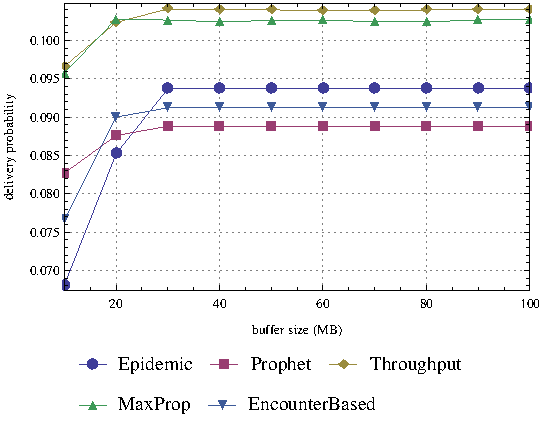
\includegraphics[width=0.32\linewidth]{paper-data/25_delivery_buffer}}
\subfigure[simulation time = 25\%\label{25_avgLatency_buffer}]
{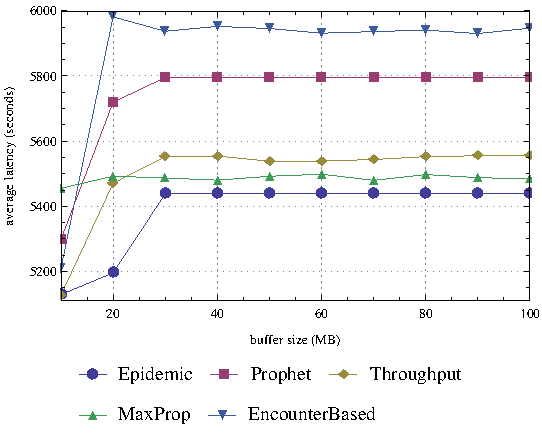
\includegraphics[width=0.32\linewidth]{paper-data/25_avgLatency_buffer}}
\subfigure[simulation time = 25\%\label{25_overhead_buffer}]
{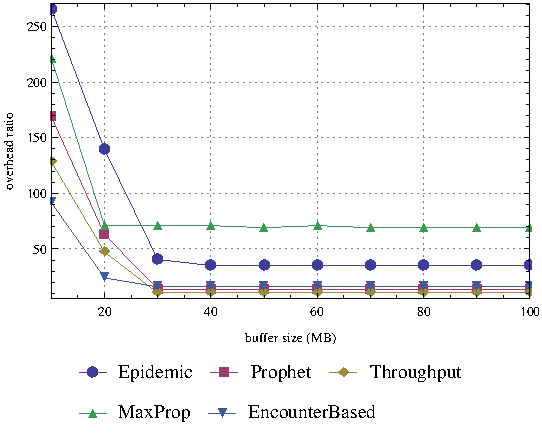
\includegraphics[width=0.32\linewidth]{paper-data/25_overhead_buffer}}
\\
\subfigure[simulation time = 50\%\label{50_delivery_buffer}]
{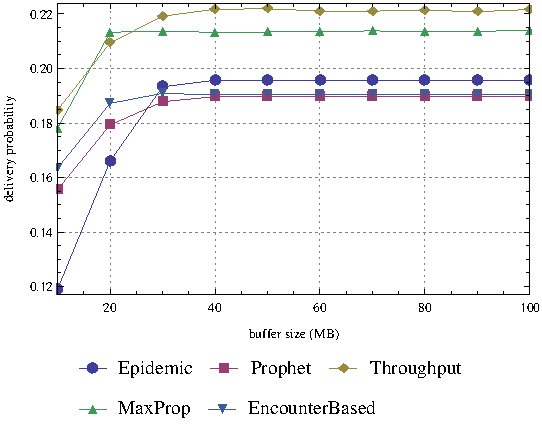
\includegraphics[width=0.32\linewidth]{paper-data/50_delivery_buffer}}
\subfigure[simulation time = 50\%\label{50_avgLatency_buffer}]
{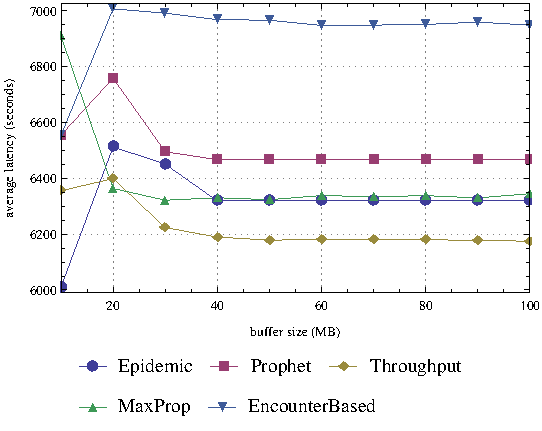
\includegraphics[width=0.32\linewidth]{paper-data/50_avgLatency_buffer}}
\subfigure[simulation time = 50\%\label{50_overhead_buffer}]
{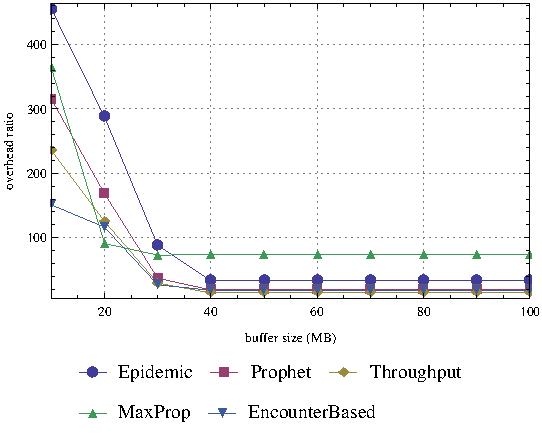
\includegraphics[width=0.32\linewidth]{paper-data/50_overhead_buffer}}
\\
\subfigure[simulation time = 75\%\label{75_delivery_buffer}]
{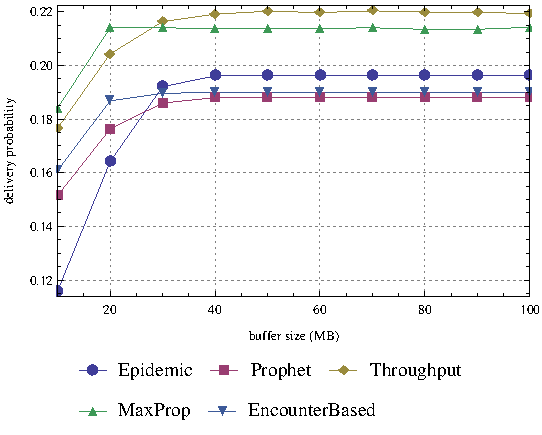
\includegraphics[width=0.32\linewidth]{paper-data/75_delivery_buffer}}
\subfigure[simulation time = 75\%\label{75_avgLatency_buffer}]
{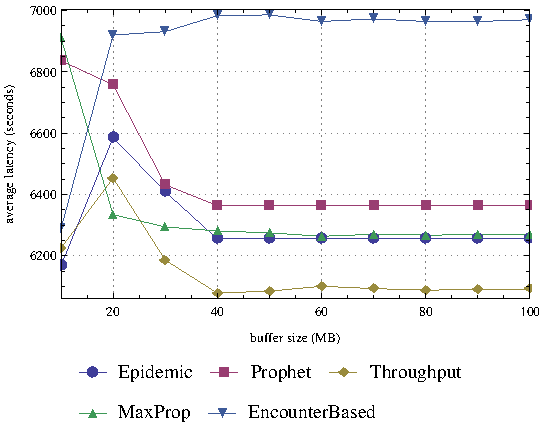
\includegraphics[width=0.32\linewidth]{paper-data/75_avgLatency_buffer}}
\subfigure[simulation time = 75\%\label{75_overhead_buffer}]
{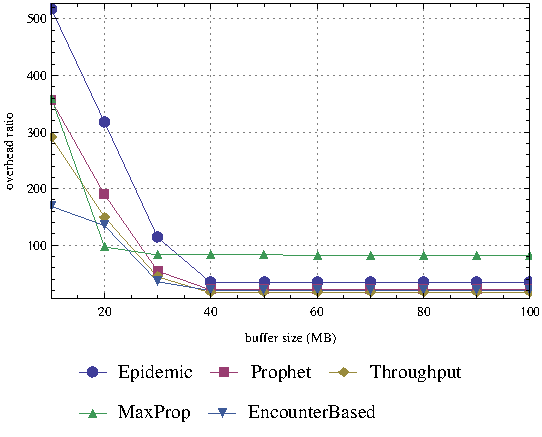
\includegraphics[width=0.32\linewidth]{paper-data/75_overhead_buffer}}
\\
\subfigure[simulation time = 100\%\label{100_delivery_buffer}]
{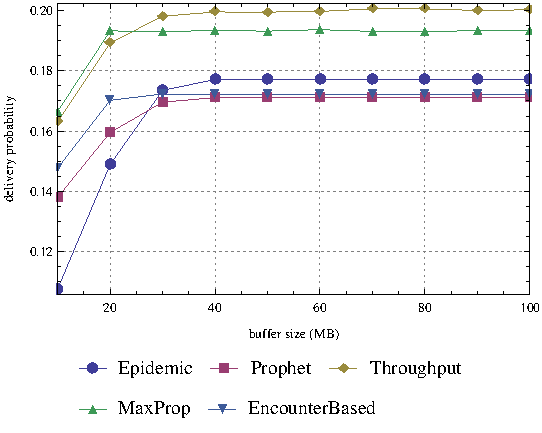
\includegraphics[width=0.32\linewidth]{paper-data/100_delivery_buffer}}
\subfigure[simulation time = 100\%\label{100_avgLatency_buffer}]
{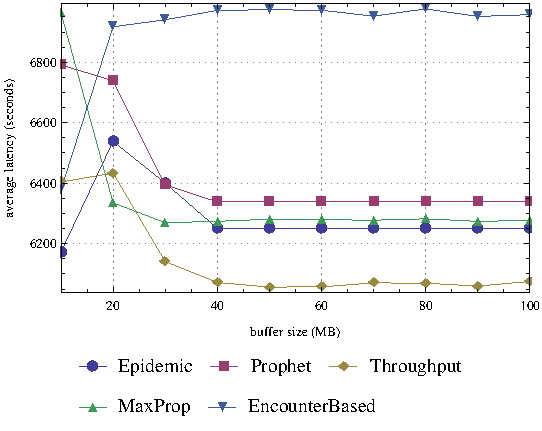
\includegraphics[width=0.32\linewidth]{paper-data/100_avgLatency_buffer}}
\subfigure[simulation time = 100\%\label{100_overhead_buffer}]
{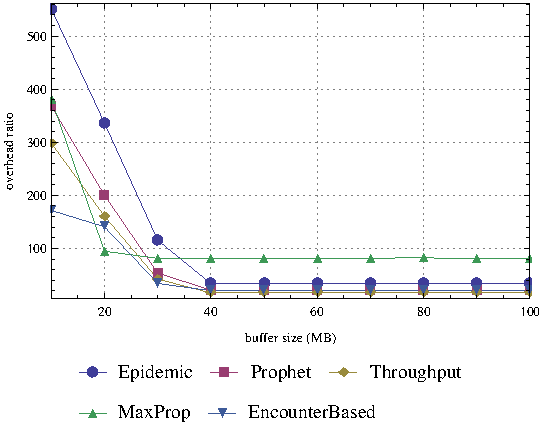
\includegraphics[width=0.32\linewidth]{paper-data/100_overhead_buffer}}
\caption{[\emph{Cambridge-iMote}] 不同仿真时间,改变节点缓存大小}
\label{fig:chap4_trace_buffer}
\end{figure*}

如\figurename~\ref{fig:chap4_trace_buffer}所示,结果表明本章中改进PRoPHET后的协议Throughput,在投递率及投递时延方面的性能表现强于PRoPHET以及Epidemic协议,且能够一定程度上降低网络开销。尽管与MaxProp算法相比,本章算法Throughput在投递率方面优势不大,然而Throughput协议在其余两方面性能表现,即投递时延和网络开销,要强于MaxProp协议。从\figurename~\ref{fig:chap4_trace_buffer}(a), \ref{fig:chap4_trace_buffer}(d), \ref{fig:chap4_trace_buffer}(g)和\ref{fig:chap4_trace_buffer}(j)可以看出,随着仿真时间的增加,Throughput算法改善投递率的效果亦增加。如\figurename~\ref{fig:chap4_trace_buffer}第二列所示,Throughput协议具有比PRoPHET更低的平均时延。参照\figurename~\ref{fig:chap4_trace_buffer}第三列的结果,随着仿真时间加长,Throughput协议能够很大程度上改善网络开销的性能表现。

\begin{figure*}[tbp]
\centering
\subfigure[simulation time = 25\%\label{25_delivery_ttl}]
{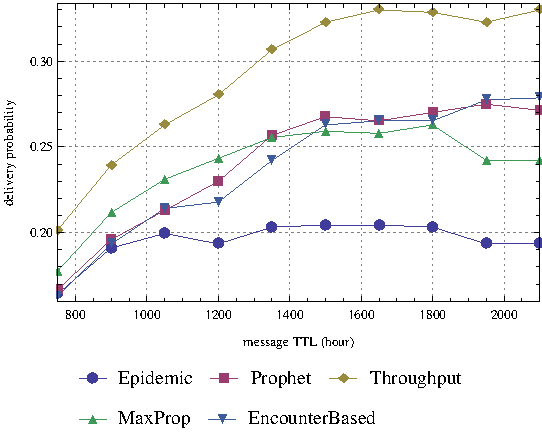
\includegraphics[width=0.32\linewidth]{paper-data/25_delivery_ttl}}
\subfigure[simulation time = 25\%\label{25_avgLatency_ttl}]
{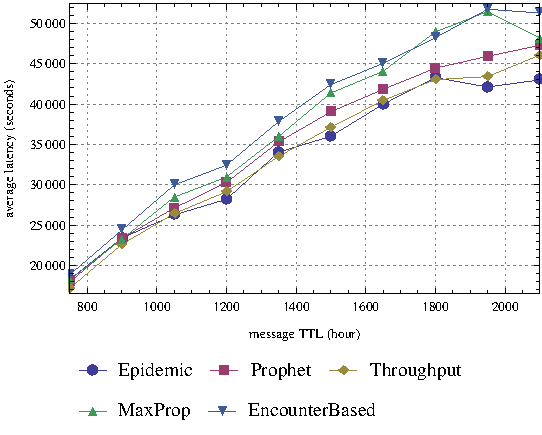
\includegraphics[width=0.32\linewidth]{paper-data/25_avgLatency_ttl}}
\subfigure[simulation time = 25\%\label{25_overhead_ttl}]
{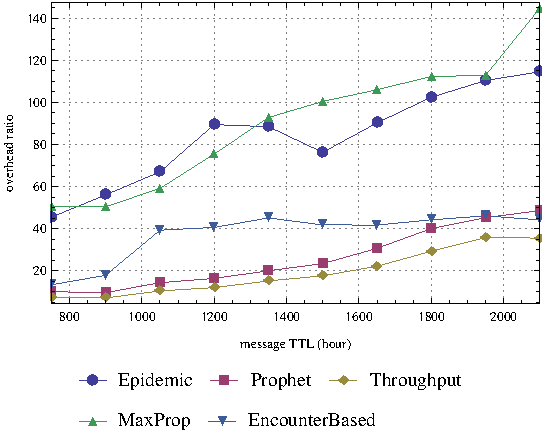
\includegraphics[width=0.32\linewidth]{paper-data/25_overhead_ttl}}
\\
\subfigure[simulation time = 50\%\label{50_delivery_ttl}]
{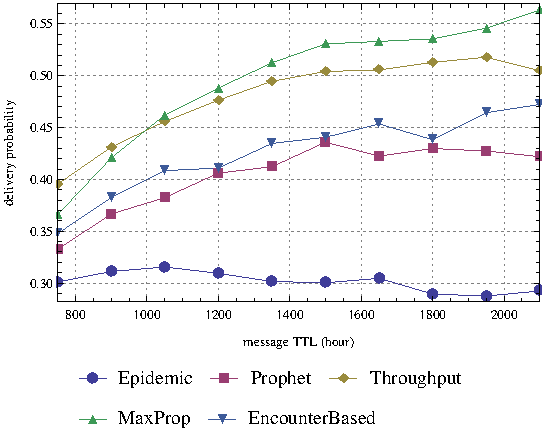
\includegraphics[width=0.32\linewidth]{paper-data/50_delivery_ttl}}
\subfigure[simulation time = 50\%\label{50_avgLatency_ttl}]
{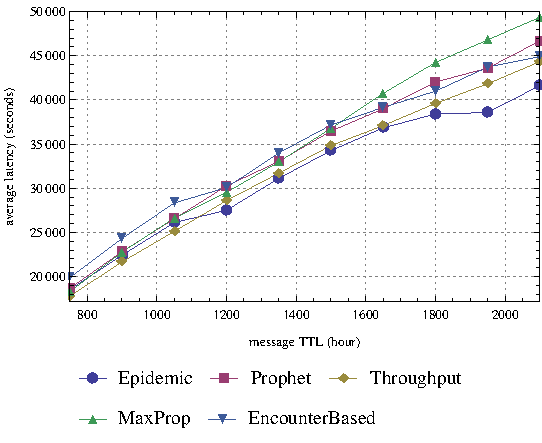
\includegraphics[width=0.32\linewidth]{paper-data/50_avgLatency_ttl}}
\subfigure[simulation time = 50\%\label{50_overhead_ttl}]
{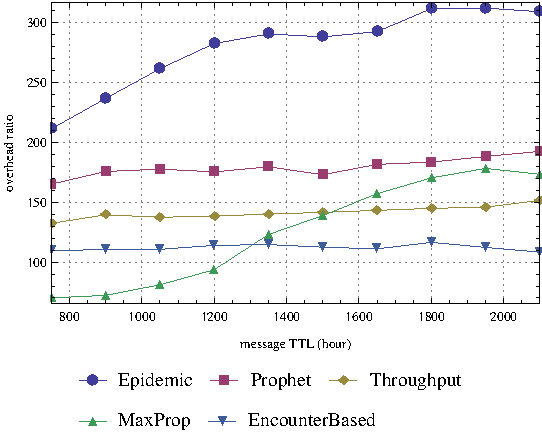
\includegraphics[width=0.32\linewidth]{paper-data/50_overhead_ttl}}
\\
\subfigure[simulation time = 75\%\label{75_delivery_ttl}]
{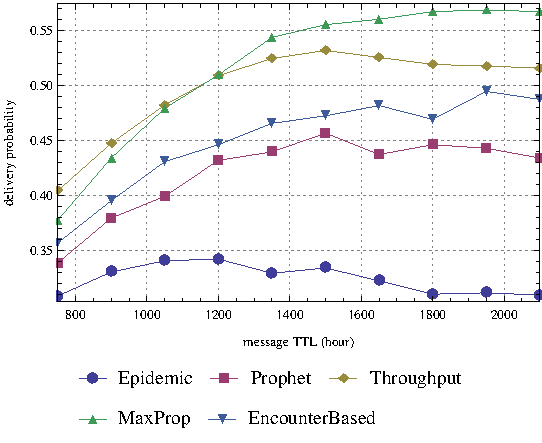
\includegraphics[width=0.32\linewidth]{paper-data/75_delivery_ttl}}
\subfigure[simulation time = 75\%\label{75_avgLatency_ttl}]
{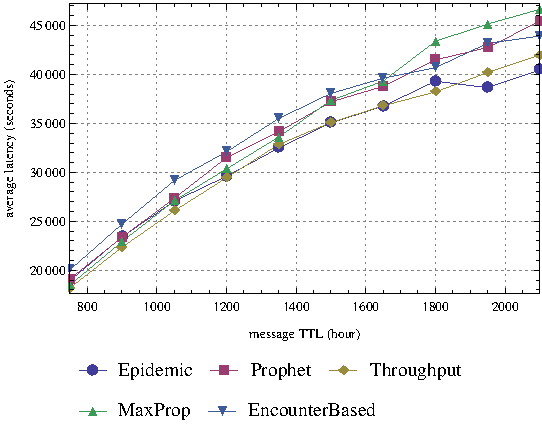
\includegraphics[width=0.32\linewidth]{paper-data/75_avgLatency_ttl}}
\subfigure[simulation time = 75\%\label{75_overhead_ttl}]
{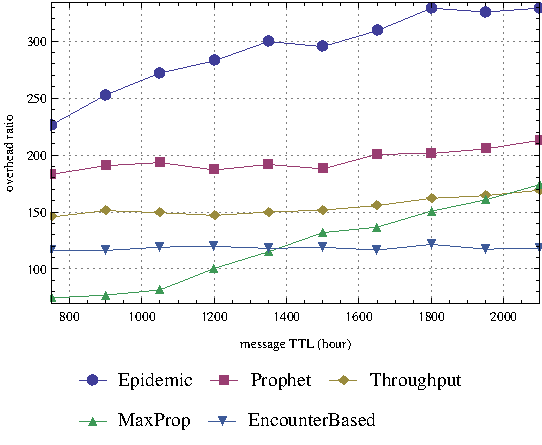
\includegraphics[width=0.32\linewidth]{paper-data/75_overhead_ttl}}
\\
\subfigure[simulation time = 100\%\label{100_delivery_ttl}]
{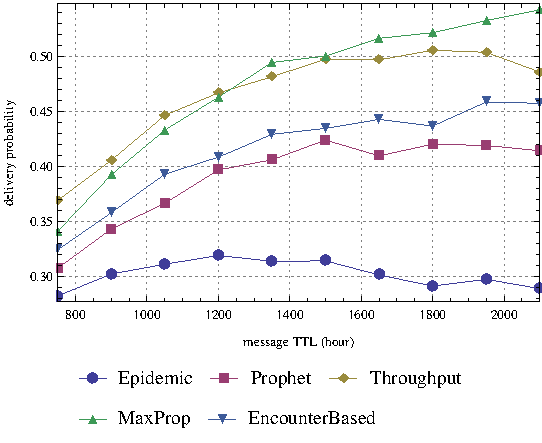
\includegraphics[width=0.32\linewidth]{paper-data/100_delivery_ttl}}
\subfigure[simulation time = 100\%\label{100_avgLatency_ttl}]
{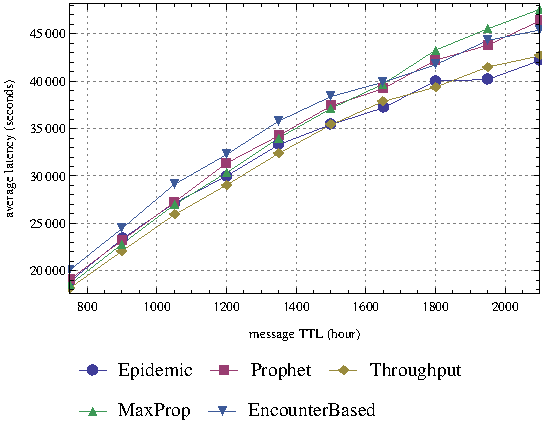
\includegraphics[width=0.32\linewidth]{paper-data/100_avgLatency_ttl}}
\subfigure[simulation time = 100\%\label{100_overhead_ttl}]
{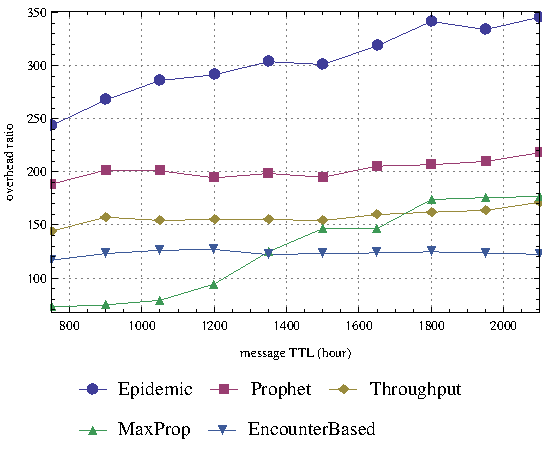
\includegraphics[width=0.32\linewidth]{paper-data/100_overhead_ttl}}
\caption{[\emph{Cambridge-iMote}] 不同仿真时间,改变消息TTL}
\label{fig:chap4_trace_ttl}
\end{figure*}

\figurename~\ref{fig:chap4_trace_ttl}的结果表明,Throughput协议在投递率以及网络开销方面的表现优于其余四种算法;在平均时延方面有微小改进。与Epidemic, PRoPHET以及EncounterBased协议相比,Throughput具有更优的性能表现。与MaxProp相比,Throughput算法在仿真时间较短时,性能表现明显好于MaxProp。该结果表明Throughput能够更快的达到算法最佳表现。



\subsection{Helsinki City Scenario仿真}

\begin{table}
\centering
\caption{Simulation settings of Helsinki City Scenario}
\label{tab:chap4_simulation_helsinki}
\begin{tabular}{
p{0.45\linewidth}<{\centering}
p{0.5\linewidth}<{\centering}
}
\hline
\textbf{parameter name} & \textbf{range(default value)} \\
\hline
pedestrians/cars & 30-90  \\
world size($m\times m$) & 4500$\times$3000  \\
initial tickets number & 6 \\
message TTL(min) & 180--425 (300) \\
simulation time(hours) & 12 \\
message size(KB) & 500--1024 \\
pedestrian buffer(MB) & 5--55 (25) \\
tram buffer(MB) & 500 \\
bluetooth range(m) & 10 \\
highspeed range(m) & 1000 \\ 
bluetooth (KBps) & 250 \\
highspeed (MBps) & 10 \\ 
pedestrian speed(m/s) & 0.5--1.5  \\
message interval(s) & 35--40 \\
\hline
\end{tabular}
\end{table}

在Helsinki City Scenario\cite{Keranen2010}中,节点持有移动设备,并利用蓝牙接口进行通信,数据率设为250 KBps,传输范围直径设为10 m。在该场景中,每个节点的初始缓存大小设为较小的值,在5 M到55 M之间变动。地图中设有六辆电车沿着指定路径移动,并且配有额外的高速通信接口,数据率为10 MBps,传输直径为1000 m 电车之间可以使用该接口进行通信。其余仿真设置如\tablename~\ref{tab:chap4_simulation}

\begin{figure}[htbp]
\centering
\subfigure[number of pedestrians/cars = 30\label{helsinki/30_delivery_buffer}]
{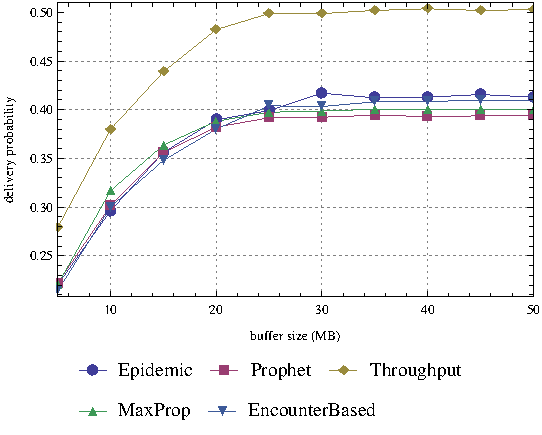
\includegraphics[width=0.32\linewidth]{paper-data/helsinki/30_delivery_buffer}}
\subfigure[number of pedestrians/cars = 30\label{helsinki/30_avgLatency_buffer}]
{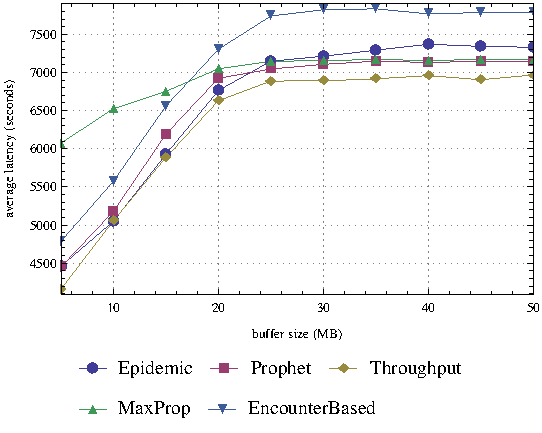
\includegraphics[width=0.32\linewidth]{paper-data/helsinki/30_avgLatency_buffer}}
\subfigure[number of pedestrians/cars = 30\label{helsinki/30_overhead_buffer}]
{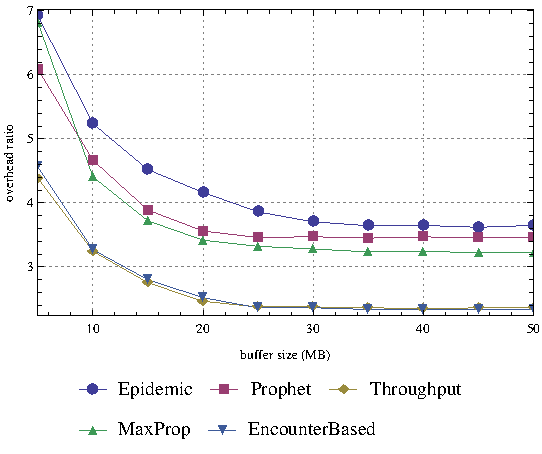
\includegraphics[width=0.32\linewidth]{paper-data/helsinki/30_overhead_buffer}}
\\
\subfigure[number of pedestrians/cars = 60\label{helsinki/60_delivery_buffer}]
{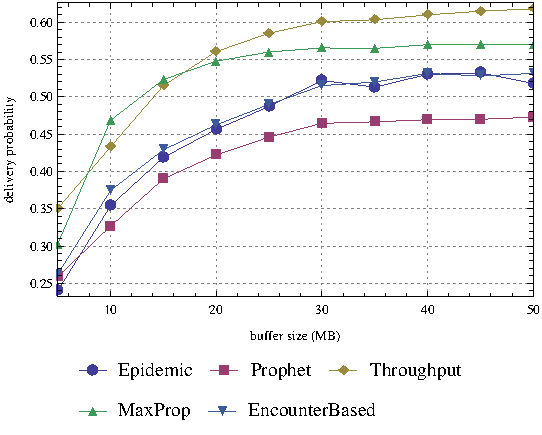
\includegraphics[width=0.32\linewidth]{paper-data/helsinki/60_delivery_buffer}}
\subfigure[number of pedestrians/cars = 60\label{helsinki/60_avgLatency_buffer}]
{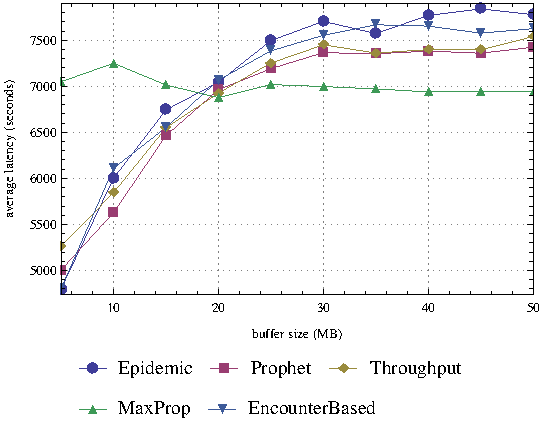
\includegraphics[width=0.32\linewidth]{paper-data/helsinki/60_avgLatency_buffer}}
\subfigure[number of pedestrians/cars = 60\label{helsinki/60_overhead_buffer}]
{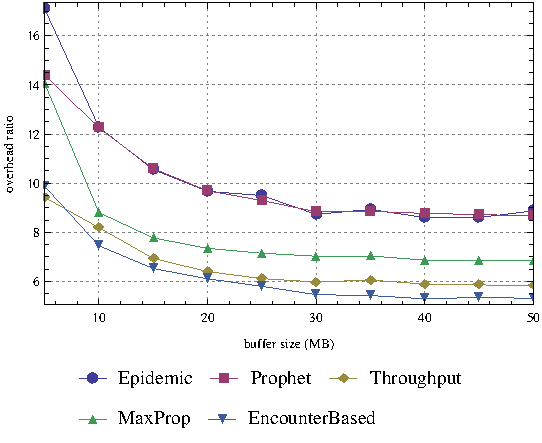
\includegraphics[width=0.32\linewidth]{paper-data/helsinki/60_overhead_buffer}}
\\
\subfigure[number of pedestrians/cars = 90\label{helsinki/90_delivery_buffer}]
{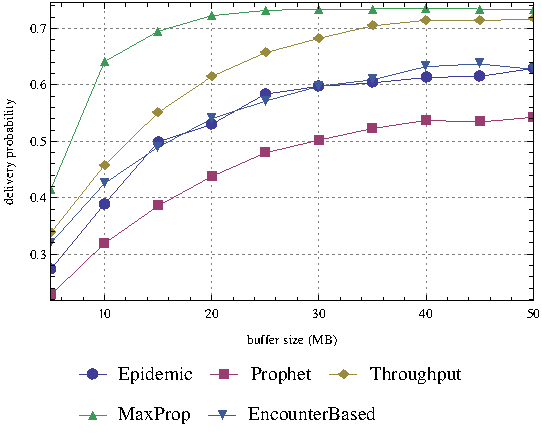
\includegraphics[width=0.32\linewidth]{paper-data/helsinki/90_delivery_buffer}}
\subfigure[number of pedestrians/cars = 90\label{helsinki/90_avgLatency_buffer}]
{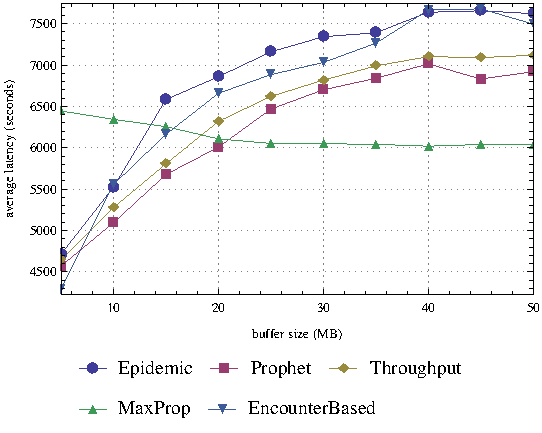
\includegraphics[width=0.32\linewidth]{paper-data/helsinki/90_avgLatency_buffer}}
\subfigure[number of pedestrians/cars = 90\label{helsinki/90_overhead_buffer}]
{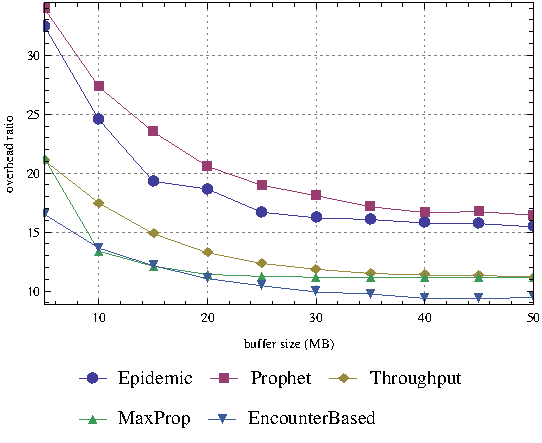
\includegraphics[width=0.32\linewidth]{paper-data/helsinki/90_overhead_buffer}}
\caption{[\emph{Helsinki City Scenario}] 不同节点数目,改变节点缓存大小}
\label{fig:chap4_helsinki_buffer}
\end{figure}

如\figurename~\ref{fig:chap4_helsinki_buffer}结果所示,Throughput路由算法在投递率上较大程度优于EncounterBased,PRoPHET以及Epidemic三种路由。随着仿真场景中行人数目以及汽车数目增加,MaxProp路由协议的性能表现逐渐好转,最终在三个指标上优于其余算法。然而当网络中不具备足够多的行人及车辆节点时,MaxProp的性能表现几乎与PRoPHET一样。在这种情况下,Throughput在三项指标上的表现全面优于MaxProp。从\figurename~\ref{fig:chap4_helsinki_buffer}(a), \figurename~\ref{fig:chap4_helsinki_buffer}(d)以及\figurename~\ref{fig:chap4_helsinki_buffer}(g)中,可以看出投递率的性能表现随着行人/汽车节点数目的增加而上升。如\figurename~\ref{fig:chap4_helsinki_buffer}第二列所示,Throughput算法与PRoPHET有几乎相同的投递时延。从\figurename~\ref{fig:chap4_helsinki_buffer}第三列可以看出,Throughput在网络开销上的改善效果较为明显。综合\figurename~\ref{fig:chap4_helsinki_buffer}所有结果来看,当节点数目较少时,Throughput具有综合最优的性能表现。

\begin{figure}[htbp]
\centering
\subfigure[number of pedestrians = 30\label{helsinki/30_delivery_ttl}]
{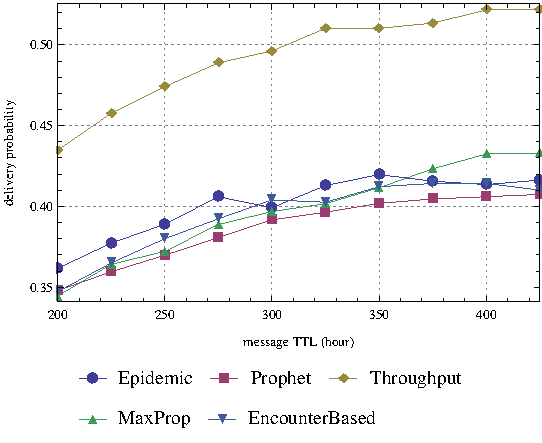
\includegraphics[width=0.32\linewidth]{paper-data/helsinki/30_delivery_ttl}}
\subfigure[number of pedestrians = 30\label{helsinki/30_avgLatency_ttl}]
{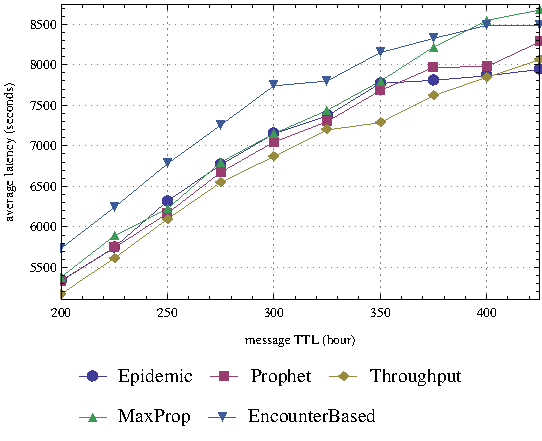
\includegraphics[width=0.32\linewidth]{paper-data/helsinki/30_avgLatency_ttl}}
\subfigure[number of pedestrians = 30\label{helsinki/30_overhead_ttl}]
{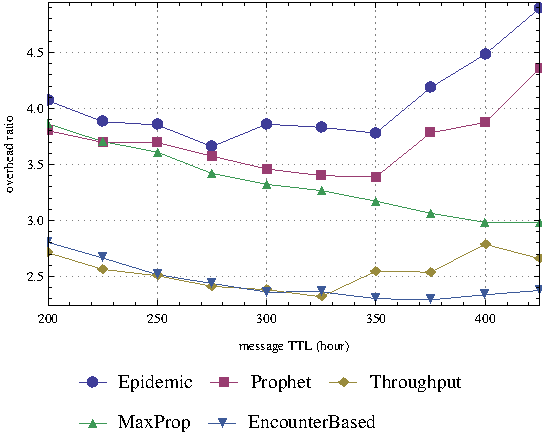
\includegraphics[width=0.32\linewidth]{paper-data/helsinki/30_overhead_ttl}}
\\
\subfigure[number of pedestrians = 60\label{helsinki/60_delivery_ttl}]
{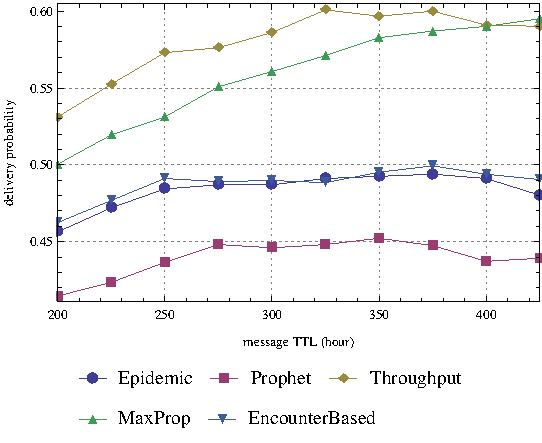
\includegraphics[width=0.32\linewidth]{paper-data/helsinki/60_delivery_ttl}}
\subfigure[number of pedestrians = 60\label{helsinki/60_avgLatency_ttl}]
{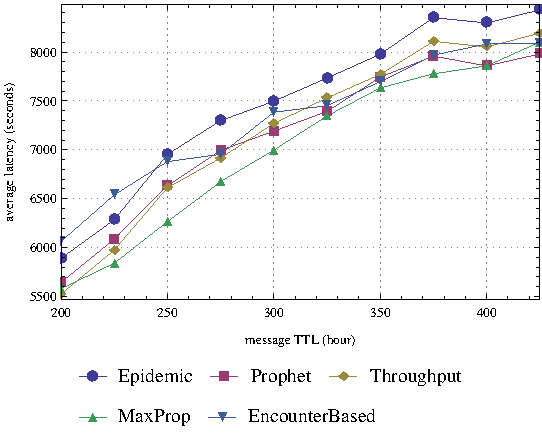
\includegraphics[width=0.32\linewidth]{paper-data/helsinki/60_avgLatency_ttl}}
\subfigure[number of pedestrians = 60\label{helsinki/60_overhead_ttl}]
{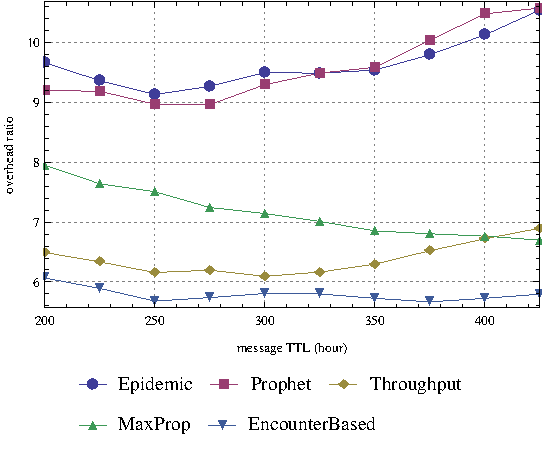
\includegraphics[width=0.32\linewidth]{paper-data/helsinki/60_overhead_ttl}}
\\
\subfigure[number of pedestrians = 90\label{helsinki/90_delivery_ttl}]
{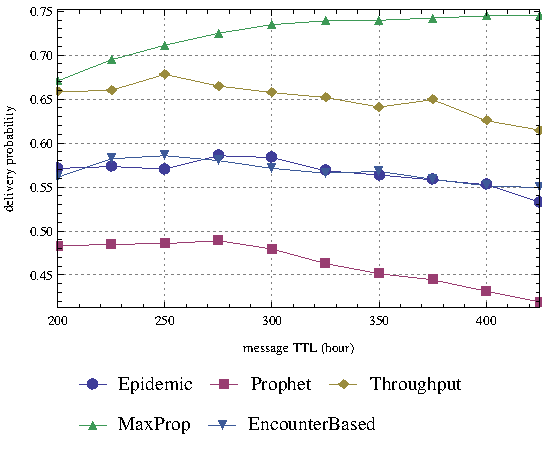
\includegraphics[width=0.32\linewidth]{paper-data/helsinki/90_delivery_ttl}}
\subfigure[number of pedestrians = 90\label{helsinki/90_avgLatency_ttl}]
{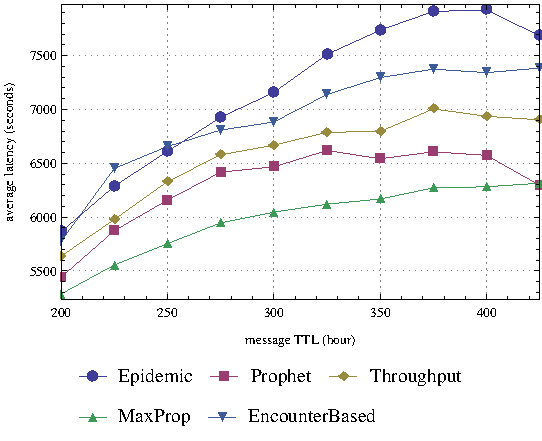
\includegraphics[width=0.32\linewidth]{paper-data/helsinki/90_avgLatency_ttl}}
\subfigure[number of pedestrians = 90\label{helsinki/90_overhead_ttl}]
{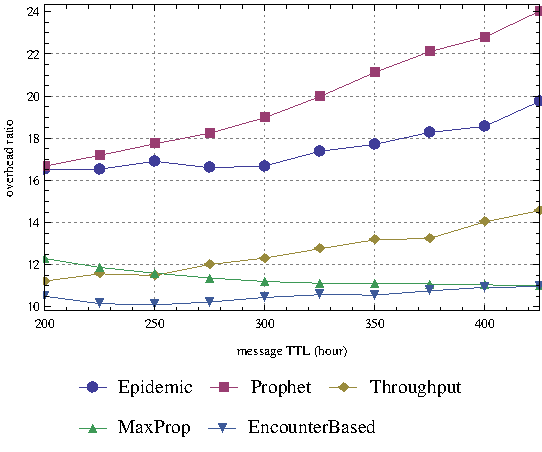
\includegraphics[width=0.32\linewidth]{paper-data/helsinki/90_overhead_ttl}}
\caption{[\emph{Helsinki City Scenario}] 不同节点数目,改变消息TTL}
\label{fig:chap4_helsinki_ttl}
\end{figure}

\figurename~\ref{fig:chap4_helsinki_ttl}展示的结果与\figurename~\ref{fig:chap4_helsinki_buffer}类似,即当节点数目较小时,Throughput算法在投递率和网络开销两个指标上优于其它四种路由算法;在投递时延上有微小优势。总而言之,若是在节点数目相对丰富,网络中的节点密度较大时,应采用MaxProp算法。当网络中节点较为稀疏时,采用Throughput算法能获得更好的性能表现。


\section{本章小结}
\label{chap4:本章小结}


本章通过设计适用于机会路由的数据项选择机制,改进了机会路由的性能表现。其出发点在于,由于节点间带宽和接触时间受限所导致的连接有限的吞吐量会造成消息的传输失败,从而浪费了节点间宝贵的接触机会。通过定义概念“消息传输效用”,在PRoPHET的基础上加上数据项选择机制,得到改进后的路由算法Throughput。仿真结果表明,该数据项选择机制能够在消息投递率,消息投递时延,网络开销三方面较大程度的改进路由性能表现。进一步地,本章定义的“消息传输效用”概念亦可用于其它路由协议上以设计相应的数据项选择机制,该课题将作为以后的研究工作。


